%% Title: Jeliot 3 - User Guide
%% File: userguide.tex
%% Author: Timo Rongas <timo.rongas@lut.fi>
%% Last Update:
%% Last Editor:

\documentclass[a4paper,11pt,english]{article}
\usepackage{graphicx}
\usepackage[latin1]{inputenc}
\usepackage[T1]{fontenc}
\usepackage{graphicx}
\usepackage{url}
\usepackage{times}
\usepackage{geometry}
\usepackage{wrapfig}
\usepackage{subfigure}
\usepackage{colortbl}
\geometry{verbose,a4paper,tmargin=30mm,bmargin=30mm,lmargin=20mm,rmargin=20mm}

\newcommand{\jel}{Jeliot}

% Use same notation for files as for URLs
\newcommand{\file}{\url}
\newcommand{\p}[1]{\texttt{#1}}
\newcommand{\bu}[1]{\textsf{#1}}
\newcommand{\code}{\p}
\newcommand{\menu}{\bu}

\setlength{\parindent}{0pt}
\setlength{\parskip}{12pt}

% TOC depth
\setcounter{tocdepth}{2}
% Table header bg-color
\definecolor{tablebg}{rgb}{1,0.95,0.95}

\begin{document}

% ### TITLEPAGE ###
\begin{titlepage}
\begin{flushleft}
Eastern Finland Virtual University (ISVY)
\end{flushleft}
\vfill{}
\Huge{Jeliot 3 - User Guide}\\
\Large{Who, Where, and What of \jel{} -- The Algorithm Theatre}
\vfill{}
\end{titlepage}
\pagebreak
\tableofcontents
\pagebreak


% ### HELLO USER ###
\section*{Hello, User}

\begin{wrapfigure}[8]{r}{60mm}
\vspace{-13pt}
Professor: ``As I often say, what you don't find elsewhere, you can find here. What you don't find here, you can go find somewhere else.''
%\includegraphics{images/tmpwrap.eps}
\end{wrapfigure}

This is the user guide for \jel{} 3 -- the Algorithm Theatre. It answers questions like ``\textit{What does this button do?}'' and ``\textit{How do I ask user for value in \jel{}?}'', and acts as the most specific source of information on usage of \jel{}. 

If you are looking for quick start installation and animation instructions, take a look at document titled \emph{Jeliot 3 - Quick Tutorial}. In case you are looking for general guidelines and examples on how to use \jel{}, take a look at \emph{Jeliot 3 - Animation Tutorial}. Everything else you may need should be in this document.

\begin{wrapfigure}[5]{l}{40mm}
\vspace{-13pt}
Here we could have some nice drawing, maybe even saying a comment if someone can think of a comment for this bad case of noncommentable place. Ugh.
\end{wrapfigure}
% If it fits on the previous page, put it there!
%{\footnotesize \tableofcontents}
%{\scriptsize \tableofcontents}
\pagebreak

% ### INTRODUCTION ###
\section{Introduction}

% comment: ``use jeliot in the classroom to show things, no matter what language you use!''
\begin{wrapfigure}[12]{r}{50mm}
\vspace{-13pt}
comment: ``It's so simple even I can use it!'' \\ \\
comment: ``use jeliot in the classroom to show things, no matter what language you use!''
%\includegraphics{images/tmpwrap.eps}
\end{wrapfigure}

\jel{} is a program animation system intended for teaching introductory programming. Programs are animated \emph{automatically}, requiring no modifications or annotations on the part of the user. While this limits the flexibility of the animation, \jel{} is extremely simple to use so that it is easily accepted by true novices, as well as by their teachers who do not have to invest on learning how to prepare animations.

\jel{} has been written in Java to gain maximum portability. It animates programs written in Java, but this does not restrict its use solely on courses that deal with Java. It has been successfully used on courses dealing with other programming languages, e.g. PASCAL. For more information on how to use \jel{} in class room, see \cite{ronit}.

% as the same basic animations are valid for learning any language! Teacher can use ready made examples for demonstrations, as understanding the syntax of Java in such basic level should be easy for anyone knowing how to program.

% ### HISTORY ###
%\section{History}
% ### RELEASE NOTES ###
%\section{Release Notes}

% ### INSTALLATION ###
\section{Installation}

\begin{wrapfigure}[16]{l}{40mm}
\vspace{-13pt}
Professor: ``For quick start, see the quick start guide. However, 'Speed is nothing, understanding is everything''' :P \\ \\
Student: ``Source code is also available. Don't touch it! :)''
%\includegraphics{images/tmpwrap.eps}
\end{wrapfigure}

Here are the instructions for downloading and installing \jel{} 3. A quicker set of instructions, meant for users that do not need so detailed information can be found from \emph{Jeliot 3 - Quick Start Guide}. Before you start, you should check that you have any of the Java environments of version 1.4 or newer installed. To verify whether you have it not, look for command \file{java.exe} or \file{java}. If it exists, you have Java (You still need to know the version. Try running \p{java -version} on commandline, it should tell you the version). Check \url{http://java.sun.com} for information on how to install Java.

The following installation instructions are split into two parts. First one deals with installation trough \emph{\jel{} windows installer}, second with \emph{\jel{} executable distribution}. Select the one you wish to use and proceed according to appropriate set of instructions. Windows users are suggested to select the \emph{windows installer} version.

If you wish to actually use \jel{}, and not play around with the way it is created, you should pick either of the above mentioned distributions. However, for the ones interested, \emph{Binary distribution} is also available. Documentation for source code is included in the package. You need to rely on that.

% ### WINDOWS INSTALLATION ###
\subsection{Installation with Windows Installer}

These instructions describe the installation process of \jel{} with the \emph{windows installer}. This is the best way for Windows users, as it is the easiest way to install, and it creates shortcuts to Start-menu and deskop for easy running of \jel{}. 

\subsubsection{Downloading}

Go to \jel{} download-page at \url{http://www.cs.joensuu.fi/jeliot/downloads.php} and click on \emph{Jeliot 3, windows installer}. Your browser should prompt you for running/saving the file. Here you should select ``save'', although it is possible to open the file directly from the web. However, we suggest you save it to disk, should the first installation fail.

The file you get is named in the following format: \file{Jeliot3-N.exe}, where N is the version number. E.g., version 2 preview 3 would be in a file called \file{Jeliot3-2P3.exe}.

\subsubsection{Installation}

Run the \file{Jeliot3-N.exe} you just downloaded by double clicking on it. A welcome window should appear (fig. \ref{fig:wininst_1}). Click \bu{Next}. The next window prompts you for the directory you wish to install \jel{} in (fig. \ref{fig:wininst_2}. Give a directory, or leave it at the default suggestion. Click \bu{Next}. Next, you are prompted for the Start-menu folder to install \jel{} in (fig. \ref{fig:wininst_3}). Give a name for the folder, or leave it at the default suggestion. Click \bu{Next}. From the next view, you can select whether you wish to have shortcuts created (fig. \ref{fig:wininst_4}). Select atleast the Start-menu)and click \bu{Next}.

Window in figure \ref{fig:wininst_5} summarizes your selections. Click \bu{Install} to start installation (fig. \ref{fig:wininst_6}). The final window just tells us that the installation is complete. Click \bu{Finish} to exit installation. Now you are ready to start \jel{}!

\begin{figure}[htp]
\begin{center}
\subfigure[Window 1]{\label{fig:wininst_1}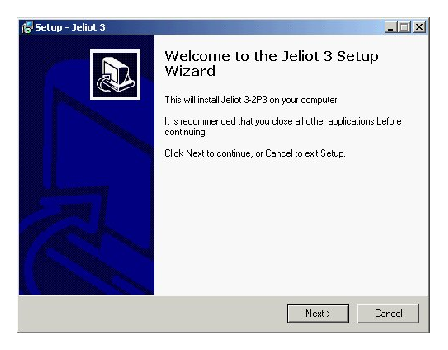
\includegraphics[]{images/wininst_1.eps}}
\subfigure[Window 2]{\label{fig:wininst_2}
\includegraphics[]{images/wininst_2.eps}} \\
\subfigure[Window 3]{\label{fig:wininst_3}
\includegraphics[]{images/wininst_3.eps}} 
\subfigure[Window 4]{\label{fig:wininst_4}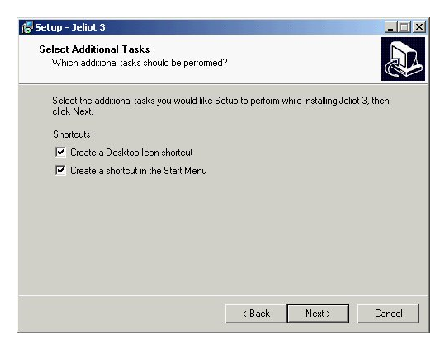
\includegraphics[]{images/wininst_4.eps}} \\
\subfigure[Window 5]{\label{fig:wininst_5}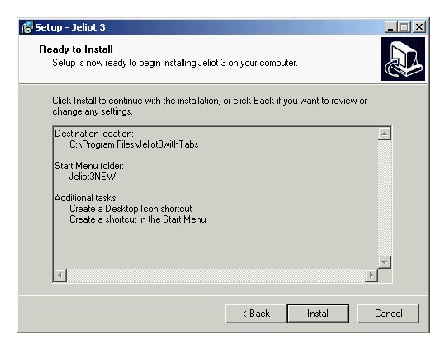
\includegraphics[]{images/wininst_5.eps}}
\subfigure[Window 6]{\label{fig:wininst_6}
\includegraphics[]{images/wininst_6.eps}}
\end{center}
\label{fig:wininst_img}
\caption{Screenshots of the installation process}
\end{figure}

\subsubsection{Running}

If the installation with the Windows Installer finished correctly, and you selected the options for creating the Start-menu shortcuts, you should have \jel{} available in your Windows Start menu under folder with the name you entered during the installation. Depending on your selections, you might also have a shortcut on your desktop. Just select either one, and \jel{} should fire up. If the installer failed to insert the shortcuts, you can start \jel{} by doubleclicking on \file{Jeliot.bat} in the directory you installed \jel{} into. If you encounter problems, check the running instructions of \emph{executable distribution} for help.

Now \jel{} should be running on your screen looking like the one in figure \ref{fig:startup}.

\begin{figure}[ht]
\begin{center}
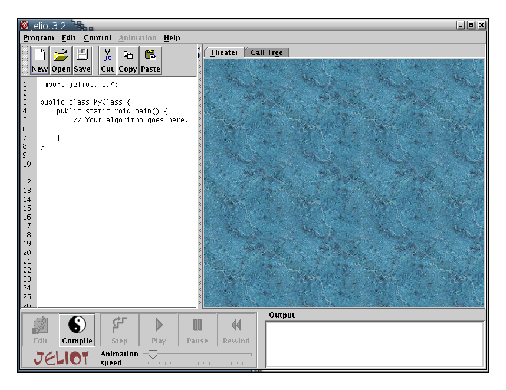
\includegraphics{images/startup.eps}
\caption{\label{fig:startup}First view of \jel{}.}
\end{center}
\end{figure}


% ### INSTALLATION WITH EXECUTABLE DISTRIBUTION ###
\subsection{\label{geninst}Installation of Executable Distribution}

This set of instructions should guide you through the installation of \jel{} under Windows, Linux, *nix or any other operating system that has a working Java environment. In case of the more extreme OSs, we trust that you know what you're doing. In case there is difference between what you are supposed to do in OSs, Windows users should check option (1) and others option (2).

\subsubsection{Downloading}
Go to \jel{} download-page at \url{http://www.cs.joensuu.fi/jeliot/downloads.php} and click on \emph{\jel{} 3 executable distribution (zipped file)}. Your browser should prompt you for opening/saving the file. Here you should select ``save'', although it is possible to open the file directly from the web if your system is properly configured. For the sake of generosity, we suggest you save the file to disk. 

The file you get is named in the following format: \file{Jeliot3-N.zip}, where N is the version number. E.g., version 2 preview 3 would be in a file \file{Jeliot3-2P3.zip}.

\subsubsection{Uncompressing}

Uncompressing the file you have just fetched from the web will result in few files and some subdirectories. First, you should create a directory for Jeliot, for example \file{c:\jeliot\} (Windows) or \file{/home/user/jeliot/} (Linux/*nix) depending on your operating system and access to it. Any folder or directory is ok, as long as you know where it is. Your unzipping program might also be able to create a directory for the files.

Next, decompress the \file{Jeliot3-N.zip} to the previously created directory using

\begin{enumerate}
\item WinZip, or some similar tool in Windows (doubleclick on the \file{Jeliot3-N.zip} file and select ``extract'' from the program. Select the directory that you just created as the target.
\item command \p{unzip Jeliot3-N.zip} in Linux/*nix environment. Note that this command will uncompress the files to the directory you are in, and will need the file \file{Jeliot3-N.zip} in the same directory. Specify the full path to uncompress the packet from elsewhere, and use -d option to specify the target directory.
\end{enumerate}

Now you should have \jel{} uncompressed on your disk. To verify, you can check that files \file{jeliot.jar}, \file{jeliot.bat}, \file{jeliot.ico}, \file{license.txt} and subdirectories \file{images}, \file{examples} and \file{docs} exist in the directory you created.

\subsubsection{Running}

To run \jel{}, 

% Student saying something about creating a shortcut!
% Or/and something about forgetting the installation directory -> search for jeliot.jar

\begin{enumerate}
\item in Windows, you can use \file{jeliot.bat}. Double click on it the start \jel{}. It might be a good idea to create a shortcut for \file{jeliot.bat} with \file{jeliot.ico} icon.
\item in Linux/*nix, you should give the command \p{java -jar jeliot.jar} in the directory where \jel{} was extracted. Actually, this is exactly what \file{jeliot.bat} does.
\end{enumerate}

Now you should have \jel{} running on your screen. Figure \ref{fig:startup} shows the startup state of \jel{}.

% ### GUI ###
\section{Graphical User Interface}

\jel{} 3 is always used through its graphical user interface (GUI). A screenshot of the \jel{} GUI is shown below in figure \ref{fig:gui}. In this chapter we go through the different parts of the GUI, one by one, describing their meaning and behavior. 

\begin{figure}[ht]
\begin{center}
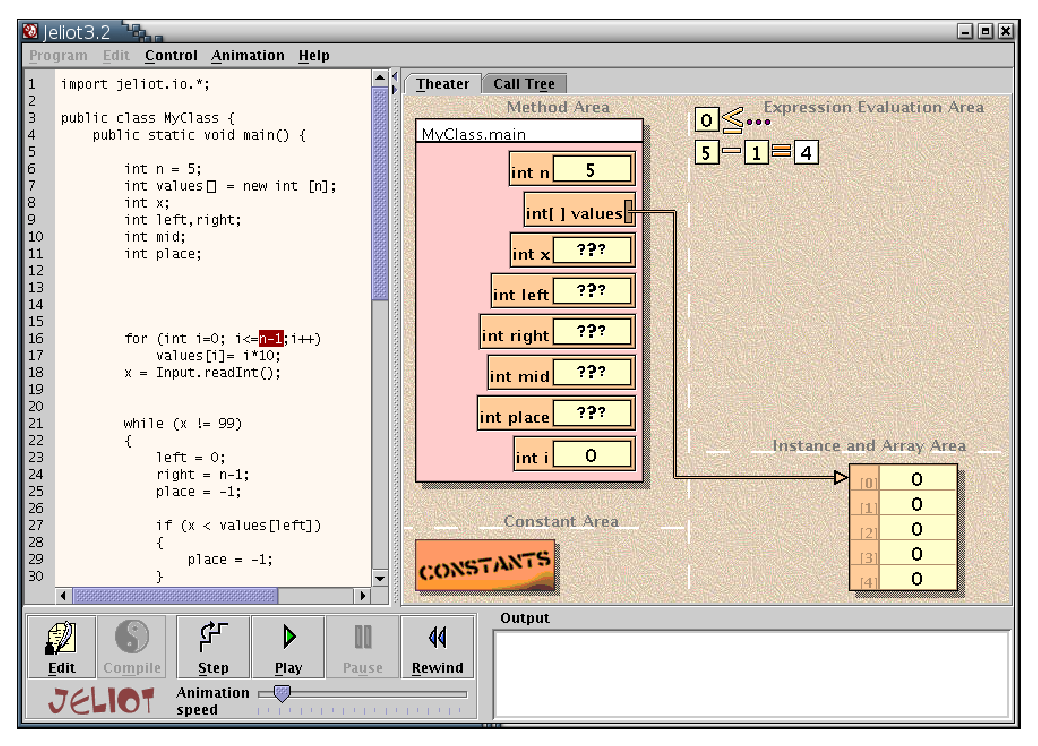
\includegraphics{images/wholegui.eps}
\caption{\label{fig:gui}Screenshot of \jel{} GUI.}
\end{center}
\end{figure}

\subsection{Source Frame}

The frame on the left hand side of the screen, consisting of linenumbered text-area, is called the source frame. When you open or create a new file, it will be opened to the source frame for editing. Clicking on \bu{Compile} will remove the editing toolbar on the top, switch the source frame to uneditable mode and slide open the curtains on animation frame. After animation, clicking on \bu{Edit} will return the source frame to editing state.

During animation, the code that is currently being animated is highlited in the source frame. For example, while in figure \ref{fig:gui} the animation frame shows \p{n-1} being calculated, the same operation is highlited in the source frame. Another example: While entering a loop, animation frame gives a message about it, and source frame will highlite the whole area of loop. You will get the hang of it when you see it happening.

\subsection{Animation Frame}

Animation frame is the main area of \jel{}. This is where all the interesting animation takes place. While in editing state, it is covered with a blue curtain. When you move to animation state, the curtain slides open and reveals a light brown background. When you start the animation, the frame is divided into four separate areas with dashed white lines. The areas in left-right, top-bottom order are \emph{Method Area}, \emph{Expression Evaluation Area}, \emph{Constant Area}, and \emph{Instance and Array Area}.

\emph{Method Area} holds activation frames for all the methods that are currently being processed. When there is nothing left in \emph{Method Area}, there is nothing left to animate. Activation frames are displayed as boxes, that hold variables inside, drawn as subboxes. Return values are animated with a larger box holding the value inside. For variables of primitive or \code{String} type, the value is displayed adjacent to the name, others are shown as links to \emph{Instance and Array Area}, or electrical ground symbol in case they are \code{null}.

\emph{Expression Evaluation Area} is just what the name says, area for evaluationg expressions. Whatever instruction needs to be executed, it is always displayed here. Information on the results of evaluting the expressions are also shown here, as well as the dialog boxes for user input.

Whenever any literals are needed by the code, they are brought to the animation from the \emph{Constants box} from \emph{Constant Area}. This applies for all literals, no matter what type they are.

Finally, the \emph{Instance and Array Area} holds dynamically reserved objects, such as instances of classes and arrays. These are connected to activation frames in \emph{Method Area} by links.


%COLOR CODING -- some wiser way to show this would be nice -- ok already
Objects in the Animation Frame follow the following color coding:

\begin{table}[ht]
\begin{center}
\caption{\label{tbl:colors}Color legend for animation frame.}
\begin{tabular}{l|l|l|l}
\hline
\textbf{Object} & \textbf{Color} & \textbf{Object} & \textbf{Color} \\
\hline
Methods & Pink box with white header &
Long & Light Green \\
Floats & Purple &
Strings & Red \\
Integers & Brown &
Doubles & \textbf{What is this color?} \\
Chars & Green &
Class Objects & Yellow \\
\hline
\end{tabular}
\end{center}
\end{table}

\subsection{Call Tree}


Call tree displays the executed function calls and their return values as a tree, \p{className.main()} being the natural root node. You can view the call tree by clicking on \bu{Call Tree} tab at the top of animation frame. The call tree is then displayed at the place of animation. Switching back to animation happens by clicking on \bu{Theater} tab. You can switch between these displays whenever you wish. However, dialog boxes will only appear on theater display. You should remember this, if you wish to follow execution from call tree view. Example of Call Tree is shown in figure \ref{fig:calltree}.

\begin{figure}[ht]
\begin{center}
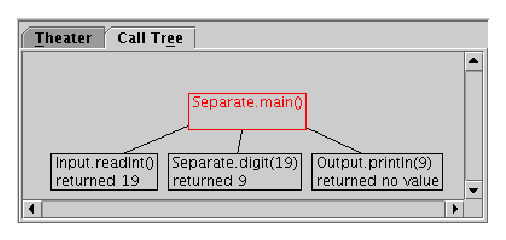
\includegraphics{images/calltree.eps}
\caption{\label{fig:calltree}Example view on call tree.}
\end{center}
\end{figure}

\subsection{\label{menus}Menus}


%Menus in \jel{} are quite self-explanatory. \menu{Program} holds commands for file operations, with \menu{Exit} as an addition. \menu{Edit} has the clipboard-functions and a \menu{Select All} button. Most of the commands from these two menus can be found from the toolbar at the top of source frame (figure \ref{fig:menutoolbar}). You can check their meaning from the next section.}

Menus in Jeliot are quite self-explanatory. \menu{Program} menu holds commands for file operations \menu{new}, \menu{open}, \menu{save}, \menu{exit} and \menu{Edit} menu holds the clipboard functions \menu{cut}, \menu{copy}, \menu{save} and \menu{select all}. Quick summary of what these commands do is shown in table \ref{tbl:fileandedit}. You can find most of the commands also in the Toolbar on top of the source frame.

\begin{table}[ht]
\begin{center}
\caption{\label{tbl:fileandedit}File and Edit operations.}
\begin{tabular}{l|p{100mm}}
\hline
\textbf{Command} & \textbf{Description} \\
\hline
\menu{New} & Inserts an empty template to source frame. \\
\menu{Open} & Opens a dialog for selecting a file to open to source frame. \\
\menu{Save} & Saves the code in source frame to given file. \\
\menu{Exit} & Exits from \jel{}. \\
\menu{Cut} & ``Cuts'' the selected text away from source frame, and places it on the clipboard. \\
\menu{Copy} & Copies the selected text from source frame to clipboard. \\
\menu{Paste} & Puts the content of clipboard to the source frame, starting from the row where the cursor is. \\
\menu{Select All} & Selects everything in source frame. \\
\hline
\end{tabular}
\end{center}
\end{table}

\menu{Control} menu holds \menu{Edit} and \menu{Compile} commands. \menu{Animation} menu holds command for controlling the flow of animation. Again, most of the commands in these two menus can be found from the toolbar at the bottom of the screen (figure \ref{fig:animation_control}) . Check the meanings of common commands from sections \ref{edit_and_compile} and \ref{animation_controls}.

In addition to the commands that are also located in the toolbar, the \menu{animation} menu holds two important commands: \menu{Pause on message} and \menu{Run until...}. The first is a checkbox, that will stop animation on any message (such as \textit{``continuing for loop''}) if it is set. The second will ask for a linenumber, and set a breakpoint there. When execution comes to this line, it is paused.

Note that \menu{Animation} menu is disabled while you are in editing state. In the same way \menu{Program} and \menu{Edit} menus will be disabled in animation state. 

\menu{Options} holds different options that are created for special situations:
\begin{itemize}
\item \menu{Save Files In Unicode}: If you experience problems with native characters
either when saving and loading files or during visualization, set this option on.

\item \menu{Save On Compilation}: Save the source file automatically before compilation.

\item \menu{Show Strings as Objects}: Changes the visualization of a String value to be an object.

\item \menu{Do Garbage Collection}: Enables garbage collection during the program visualization.
This is very useful when Strings are showns as objects because otherwise screen can be cluttered.

\item \menu{Ask For Command Line Parameters}: When the animation starts, you will be asked
for parameters for the method called.

\item \menu{Ask For Method}: When the animation starts, you will be asked for a method name
to call instead of the main method.

\item \menu{Use Null Parameter To Call Main}: If checked, the main method will be called 
with a null parameter; this avoids animating the creation of an empty array.

\item \menu{Ask Questions During Animation}: Whenever an expression is to be evaluated, a 
popup window will ask for the result. However, currently questions are generated
only for assignment statements.

\item \menu{Pause On Message}: Automatically pauses the animation to display messages
explaining its progress.

\item \menu{Show History View}: Enables or disables the generation of the history view that
shows snapshots of the previous animation in the theater. Note that the generation of
the history images takes some time and might slow down the visualization. If the animation
is too slow disable this option.

\item \menu{Select Font Of Code}: Select the font for the code editor.

\end{itemize}

Last menu is \menu{Help}. There you can find information on \jel{} (\menu{About}) and the \menu{Help} document. Help document is opened on its own window when you select it from the menu, or press \bu{F1} on your keyboard.

\subsection{Toolbar Buttons}
\label{toolbar}

While in edit state, there is a detachable\footnote{\emph{detachable} meaning a toolbar that can be drawn out of its place and relocated elsewhere by dragging it with a mouse.} toolbar with file and clipboard commands on the top of the source frame (figure \ref{fig:menutoolbar}). These work in the same way as the commands in the \menu{Program} and \menu{Edit} menu do. When you compile your code, the toolbar is hidden beneath the source frame, or just disabled in case you have detached it and left it in its own window.

\begin{figure}[ht]
\begin{center}
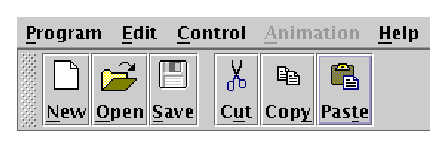
\includegraphics{images/menu_toolbar.eps}
\caption{\label{fig:menutoolbar}Program menus and File and Clipboard operations toolbar.}
\end{center}
\end{figure}

\subsection{Edit and Compile}
\label{edit_and_compile}

The toolbar shown in figure \ref{fig:animation_control} has buttons called \bu{Edit} and \bu{Compile}. It is located in the lower left corner of the window. With these buttons you control whether \jel{} is in animation or editing state. From the editing state, you can start animating by clicking on \bu{Compile}. You can return to edit the code at any time from animation state by selecting \bu{Edit}.

\begin{figure}[ht]
\begin{center}
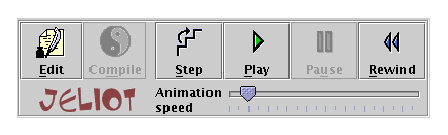
\includegraphics{images/animation_controls.eps}
\caption{\label{fig:animation_control}Edit, Compile and Animation Control toolbar.}
\end{center}
\end{figure}

\subsection{Animation Controls}
\label{animation_controls}
The animation can be controlled by the VCR-like buttons (figure \ref{fig:animation_control}) on the lower right corner of the \jel{} window. Have a look at the information on \menu{Animation} menu in section \ref{menus} for additional control features. Table \ref{tbl:commands} describes the animation controls on the toolbar.

\begin{table}[h]
\begin{center}
\caption{\label{tbl:commands}Animation toolbar commands.}

\begin{tabular}{l|p{100mm}}
\hline
\textbf{Button} & \textbf{Function} \\
\hline
\bu{Step} & Proceeds the animation with one step with the set speed. \\

\bu{Play} & Proceeds the animation continuously with the set speed untill \bu{Pause} is clicked or the program ends.\\

\bu{Pause} & Pauses running animation to situation when you click the button. \\

\bu{Rewind} & Takes you back to the beginning of program. \\

\bu{Animation Speed} & Tune the speed of animation. Left is slower, right is faster. You can also control the speed in steps from the \menu{Animation} menu. \\
\hline
\end{tabular}
\end{center}
\end{table}

\subsection{Output Frame}

Output frame is located in the lower right corner of the screen. As you can see in figure \ref{fig:output}, it is just a white textbox, that shows the data that is outputted from the animated program. All the values that are outputted are grabbed from the animation frame by a hand coming out of the box.

\begin{figure}[ht]
\begin{center}

\includegraphics{images/output.eps}
\caption{\label{fig:output}Output box, clear option in menu and value-grabbing hand.}
\end{center}
\end{figure}

Clicking on output frame gives you a menu with single selection for clearing the screen. You can use this option at any time to erase everything in the output box.

\subsection{Error Display}

In case there is an error in the code, in most cases \jel{} will tell you about it when you click on \bu{Play} or \bu{Step} for the first time. If you are trying to use an uninitialized variable, the animation will proceed normally until the point of error, where it is stopped with en error message.

A notification on error will be displayed on animation frame. Clicking \bu{OK} will take you back to animation screen, but you cannot proceed with the animation untill you correct the faulty code. That is still your job, \jel{} will not (yet) do that for you.


\section{Java Issues}

There are two incompatibilities between \jel{} and Java.

\begin{enumerate}
\item All classes must be in a single source file.

\item For I/O, import the package \p{jeliot.io.*;} which provides the  methods\\
    \p{void Output.println()}, \p{int Input.readInt()}, \p{double  Input.readDouble()},\\
    \p{char Input.readChar()}, \p{String  Input.readString()}. Standard output is also already supported.
\end{enumerate}

\jel{} uses DynamicJava (\url{http://koala.ilog.fr/djava/}) as a front-end and thus accepts almost all Java features that you would want to use for introductory programming, however, the implementation of the animation might not animate all features. Currently, the implementation includes:

\begin{itemize}

	\item Values of type \p{String}, all primitive types and one-dimensional arrays.

	\item Static variables.

	\item Expressions including all unary and binary operations except \p{instanceof}.

	\item All the control statements (\p{if}, \p{while}, etc.).

	\item Conditional expressions (\p{exp?exp1:exp2}).

	\item Method invocation, including recursive invocation.

	\item Constructors, allocation of objects and invocation of methods on objects.

\end{itemize}

\paragraph{Not implemented:}
\begin{itemize}

	\item Super field accesses.

	\item Arrays with components of reference type (except \p{String})

	\item Two or more dimensional arrays.

	\item Array initializers.

	\item Java 2 SDK API classes' methods cannot return object (except \p{String} type) or array types (e.g. \p{object.getClass()} that returns a \p{Class} instance).

	\item The used classes hashCode() -method has to return always a unique value.

\end{itemize}

\begin{thebibliography}{[99]}
\addcontentsline{toc}{section}{References}
\bibitem{ronit}
Ronit {Ben-Bassat Levy}, Mordechai Ben-Ari, and Pekka~A. Uronen.
The {Jeliot} 2000 program animation system.
{\em Computers \& Education}, 40(1), 1-15, 2003.
\end{thebibliography}

\appendix
\newpage

% ### LICENSE ###
\addcontentsline{toc}{section}{GNU Free Documentation License (?)}
\section*{GNU Free Documentation License (?)}
\section{GNU Free Documentation License}
\addcontentsline{toc}{section}{GNU Free Documentation License}
%\label{label_fdl}

\section{GNU Free Documentation License}
\addcontentsline{toc}{section}{GNU Free Documentation License}
%\label{label_fdl}

\section{GNU Free Documentation License}
\addcontentsline{toc}{section}{GNU Free Documentation License}
%\label{label_fdl}

\input{../FDL}

\end{document}
